\appendix
\chapter{Anhang}
\section{Übersicht der Trainingseinheiten}
\label{anhang:trainingsarten}
Die Zeitspannen, die ein Belastungsbereich einnehmen darf sind in Minuten angegeben.
\newcolumntype{b}{>{\hsize=0.32\hsize}X}
\newcolumntype{m}{>{\hsize=0.11\hsize}X}
\newcolumntype{s}{>{\hsize=0.02\hsize}X}
\begin{table}[h]
    \centering
    \footnotesize 
    \begin{tabularx}{\textwidth}{|s|b|mmmmmm|}
    \hline
            \rowcolor{ctcolorgraylight} 
             & \textbf{Einheit} & \textbf{KB} & \textbf{GA}& \textbf{EB}& \textbf{SB}& \textbf{K123}   &\textbf{K45} \\  \hline
    1 & Kompensationsfahrt                  & 15-180 &         &             &        &        &           \\ \hline
    2 & Extensive Fahrt                     &        & 30-300  &             &        &        &           \\ \hline
    3 & Fettstoffwechselfahrt               &        & 60-300 &             &        &        &           \\ \hline
    4 & Intensive Fahrt                     &        & 30-60      & 15-60       &        &        &           \\ \hline
    5 & Extensive Kraftausdauerfahrt        &        & 30-60   &             &        & 15-150 &           \\ \hline
    6 & Einzelzeitfahrt                     &        & 30-60      &             & 15-60  &        &     \\ \hline
    7 & Extensives Fahrtspiel               &        & 15-240    & 15-240    &           &       &       \\\hline
    8 & Intensives Fahrtspiel               &        & 15-300    & 15-300    & 15-300    & 15-180      &    15-180   \\\hline
    9 & Intensive Kraftausdauerfahrt        &        & 30-90   &             &        &        & 15-120        \\\hline
    10& Schnelligkeitsausdauer              &        & 60-180  &             & 15-45  &        &           \\ \hline 
    11& Sprinttraining                      &        & 15-30   &             & 15-60  &        &       \\\hline           

    \end{tabularx}
    \caption{Einheiten aus allen Trainingsmethoden}
    \label{anhang:einheiten}
\end{table}
\newpage
\section{Schema anhand hierarchischer Zyklisierung}
\label{anhang:modellierung:gross}
\rotatebox{90}{\begin{minipage}{0.9\textheight}
    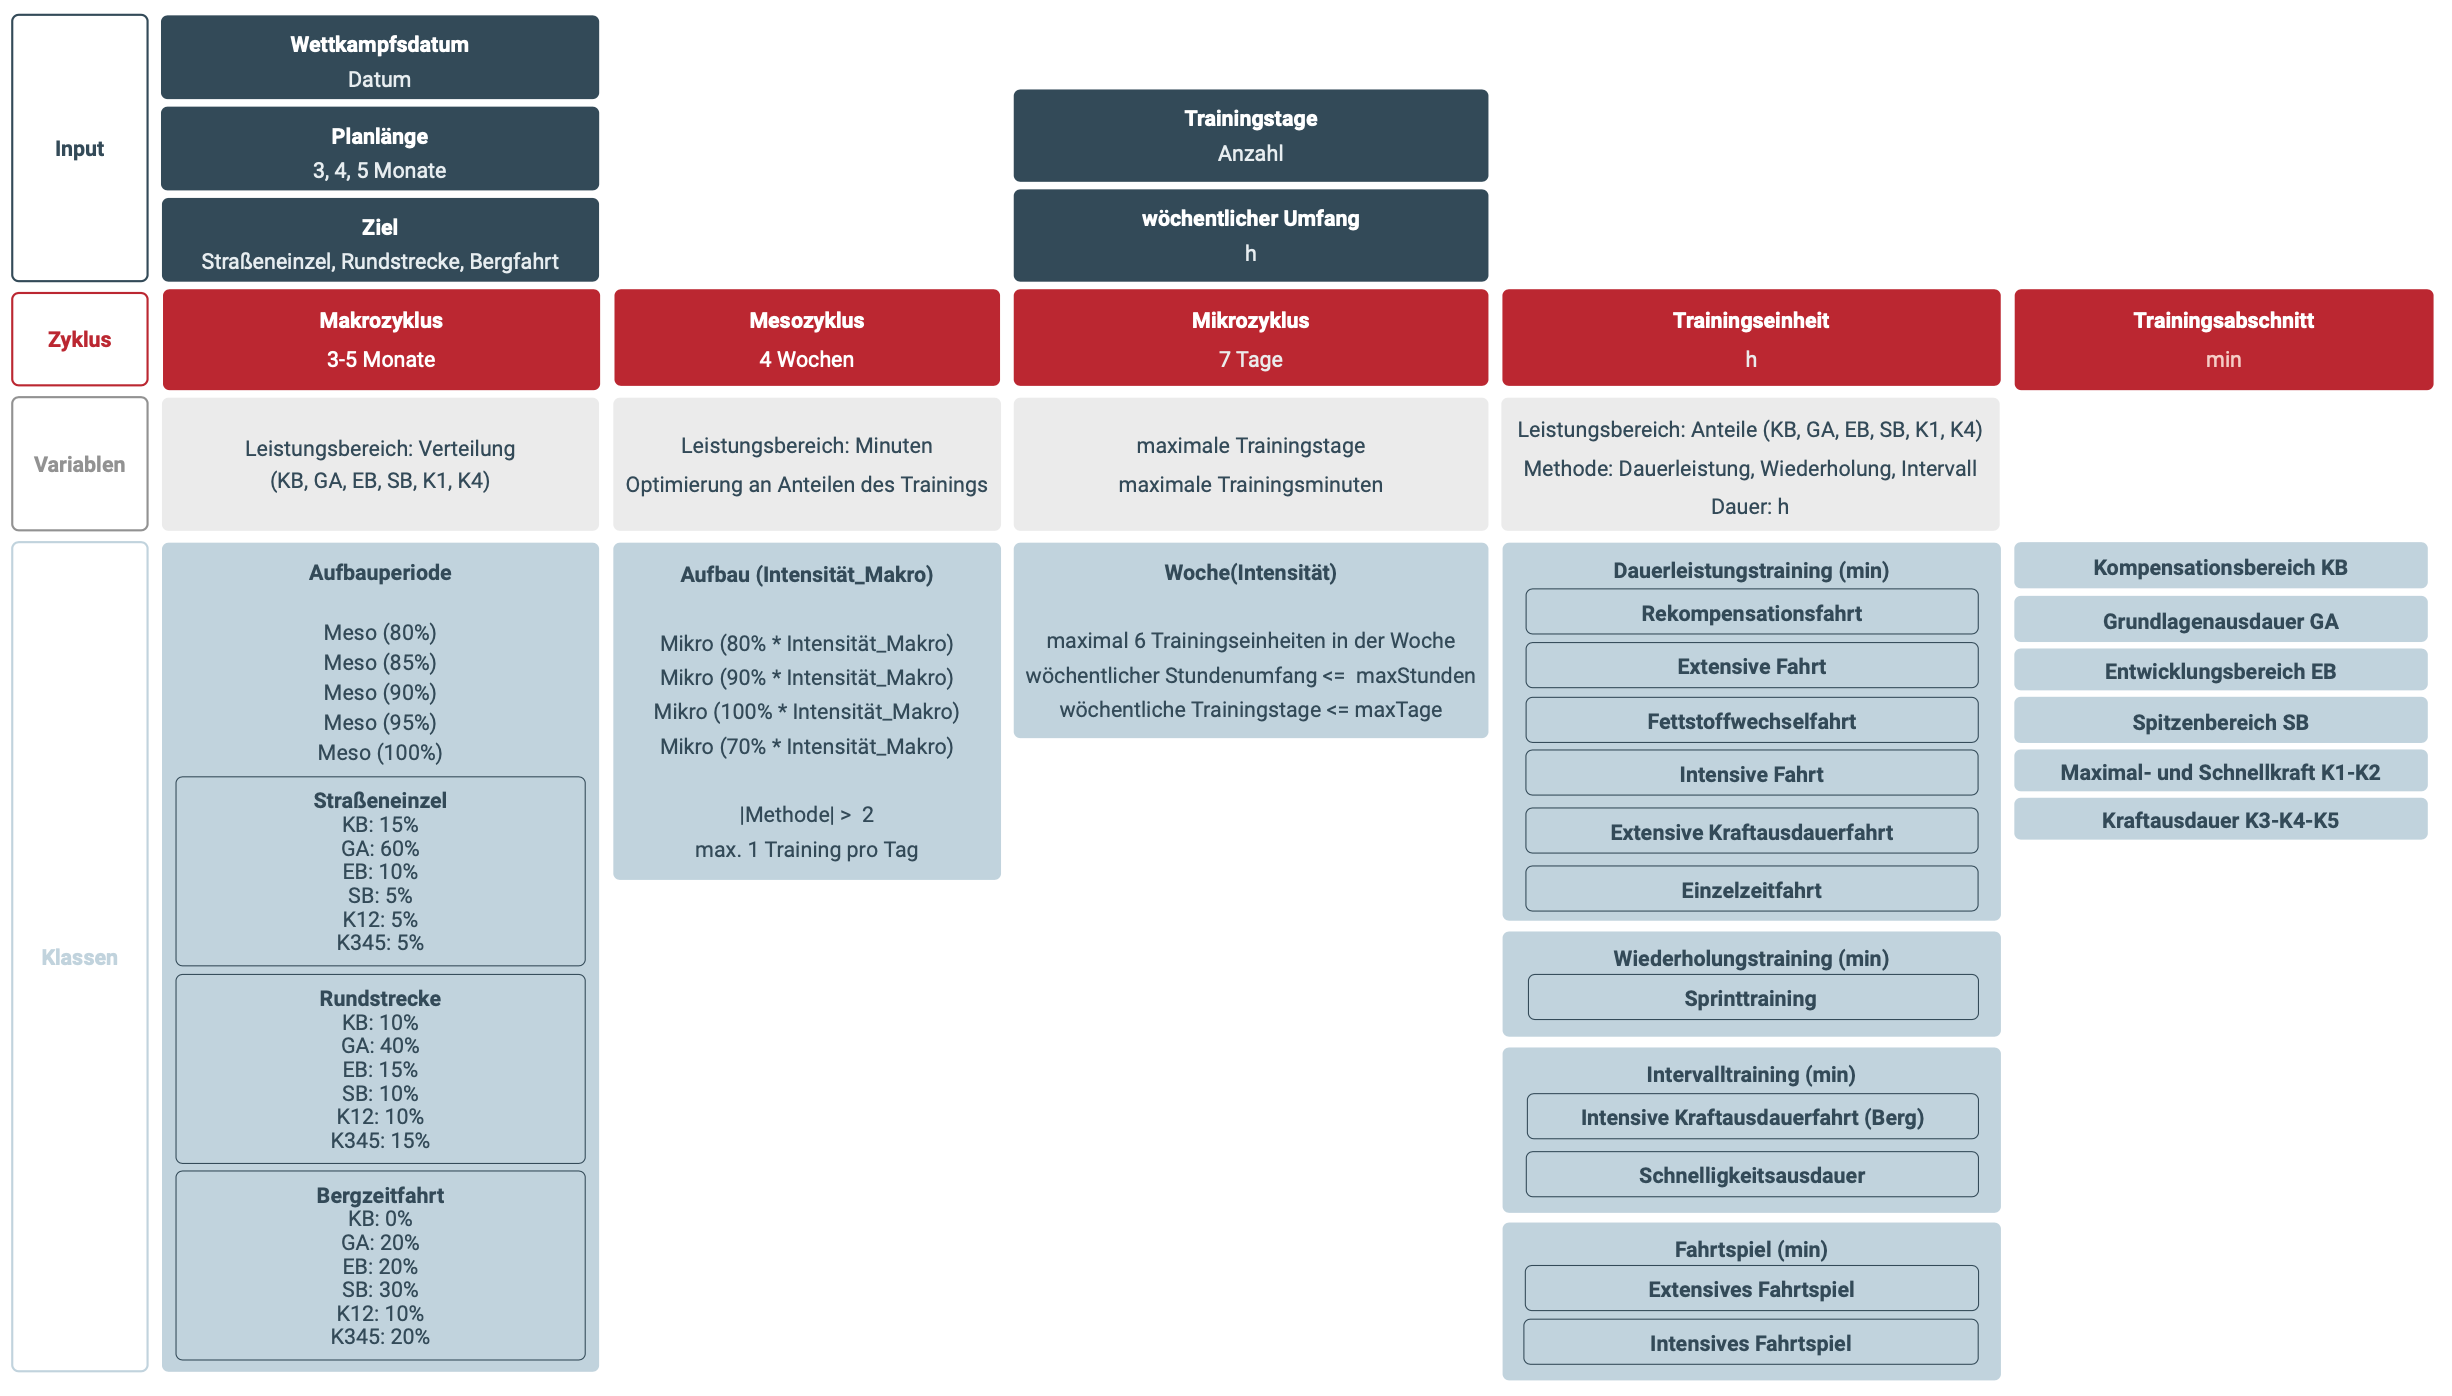
\includegraphics[width=\textwidth]{gfx/modellierung.png}
    \captionof{figure}{Schema anhand hierarchischer Zyklisierung}
    \end{minipage}
}
\newpage
\section{Mathematische Modellierung}
\label{anhang:modell}
\begin{equation*}
    \forall i \in [1, 28], min_i \mod 15 = 0
\end{equation*} 
\begin{equation*}
\begin{array}{c}
    \forall i \in [1, 28], kb_i \mod 15 = 0 \\
    \forall i \in [1, 28], ga_i \mod 15 = 0 \\
    \forall i \in [1, 28], eb_i \mod 15 = 0 \\
    \forall i \in [1, 28], sb_i \mod 15 = 0 \\
    \forall i \in [1, 28], k1_i \mod 15 = 0 \\
    \forall i \in [1, 28], k4_i \mod 15 = 0 \\
\end{array}
\end{equation*}
\begin{equation*} 
    \forall m \in ,|\{method_i = m | i \in [1, 28]\}| \geq 2
\end{equation*} 
\begin{equation*}
    \forall i = k * 7 + 1, k \in Z, \sum_{i}^{i+6} \text{duration}_i \leq max_{hours} 
\end{equation*}
\begin{equation*}
    \forall i \in \{ i = k * 7 + 1, k \in Z \}, \sum_{i}^{i+6} \text{duration}_i \leq max_{hours}
\end{equation*}
\begin{equation*}
    \forall i = k * 7 + 1, k \in Z, \sum_{i}^{i+6} \text{day}_i \leq max_{days}
\end{equation*}
\begin{equation*}
    method_i = \text{PAUSE} \Leftrightarrow minutes_i = 0
\end{equation*}
\begin{equation*}
    (method_i = \text{Dauerleistung})\Rightarrow t_i = \begin{array}{c}
            ([\![15, 180]\!], 0, 0, 0, 0, 0) \\ 
            \vee (0, [\![30, 300]\!], 0, 0, 0, 0) \\  
            \vee (0, [\![60, 300]\!], 0, 0, 0, 0) \\  
            \vee (0, [\![30, 60]\!], [\![15, 60]\!], 0, 0, 0) \\  
            \vee (0, [\![30, 60]\!], 0, 0, [\![15, 150]\!], 0) \\
            \vee (0, [\![30, 60]\!], 0, [\![15, 60]\!], 0, 0) \\  
    \end{array}
\end{equation*}
\begin{equation*}
    (method_i = \text{Fahrtspiel})\Rightarrow t_i = \begin{array}{c}
                (0, [\![15, 240]\!], [\![15, 240]\!], 0, 0, 0) \\ 
           \vee (0, [\![15, 300]\!], [\![15, 300]\!], [\![15, 300]\!], [\![0, 180]\!], [\![0, 180]\!])
    \end{array}
\end{equation*}
\begin{equation*}
    (method_i = \text{Intervall})\Rightarrow t_i = \begin{array}{c}
            (0, [\![30, 90]\!], 0, 0, 0, [\![15, 120]\!]) \\ 
        \vee (0, [\![60,180]\!], 0, [\![15, 45]\!], 0, 0)
    \end{array}
\end{equation*}
\begin{equation*}
    (method_i = \text{Wiederholung})\Rightarrow t_i = \begin{array}{c}
            (0, [\![15, 30]\!], 0, [\![15, 60]\!], 0, 0)
    \end{array}
\end{equation*}
\begin{equation*}
    \text{minimize} \sum_{m\in M} |\text{target}_m - \text{sum}_m|
\end{equation*} 
\newpage
\section{Klassendiagramm}
\label{anhang:uml}
\begin{figure}[h]
    \begin{tikzpicture}
        \umlclass[y=11.5, fill=white]{Main}{
        }{
            + monitorStats() : void \\
            + createPlan() : void \\
            + createTable(i : int) : void \\
            + createPDF(i : int) : void \\}
        \umlclass[x=8, y=11.5, fill=white]{OutputTrainingTable}{
        }{
            + displayPlan() : void \\
        }
        \umluniassoc[arg=-table , mult2=1, pos =0.95, align=right]{Main}{OutputTrainingTable}
        \umluniassoc[arg=-plan , mult2=0..1, pos =0.8, align=right]{Main}{Macro}
        
        \umlclass[y=5, fill=white, type = abstract]{Macro}{
            - sessions : ArrayList<Session> \\
            - numMonth : int \\
            - maxTrainingMinutes : int \\
            - maxTrainingDays : int \\
            - compDay : Date \\
            - ranges : HashMap<Range, Double> \\
        }{
            + solvePlan() : void \\
            \textit{+ setRanges() : void} \\
            + validateRanges() : void \\
        }
        
        \umlclass[x=8, y=5, fill=white]{Meso}{
            - model : Model \\
            - plan : Solution \\
            - startDay : Date \\
            - targetRanges : int[6] \\
            - targetMinutes : int[4] \\
            - name : IntVar[] \\
            - minutes : IntVar[] \\
            - method : IntVar[] \\
            - ranges : IntVar[][] \\    
            - distanceRanges : IntVar[] \\
            - overallDistance : IntVar \\

        }{
            - initializeModel() : void \\
            - defineConstraints() : void \\
            + solveMonth() : void \\
            + getSessions() : Session[] \\
            + getPlan() : Solution \\
        }
        \umlclass[x=8, y=-3, fill=white]{Session}{
            - name : String \\
            - minutes : int \\
            - distribution : HashMap<Range, Integer> \\
            - day : LocalDate \\
            - method : Method \\
        }{
        }
        \umlclass[x=1, y=0, fill=white]{Strasseneinzel}{}{+ setRanges() : void}
        \umlclass[x=1, y=-2, fill=white]{Rundfahrt}{}{+ setRanges() : void}
        \umlclass[x=1, y=-4, fill=white]{Bergfahrt}{}{+ setRanges() : void}
        
        
        \umlHVinherit[anchor2=-130]{Strasseneinzel}{Macro}
        \umlHVinherit[anchor2=-130]{Rundfahrt}{Macro}
        \umlHVinherit[anchor2=-130]{Bergfahrt}{Macro}
        \umluniassoc[arg=-mesos ,  mult2=3..5, pos =0.95, align=right]{Macro}{Meso}
        \umluniassoc[arg=-sessions , mult2=28, pos =0.80, align=right]{Meso}{Session}
    \end{tikzpicture}
    \caption{Klassendiagramm der vollständigen Anwendung}
    \label{fig:uml:solver}
\end{figure}

\newpage
\section{Grafische Benutzungsoberfläche}
\rotatebox{90}{\begin{minipage}{0.9\textheight}
    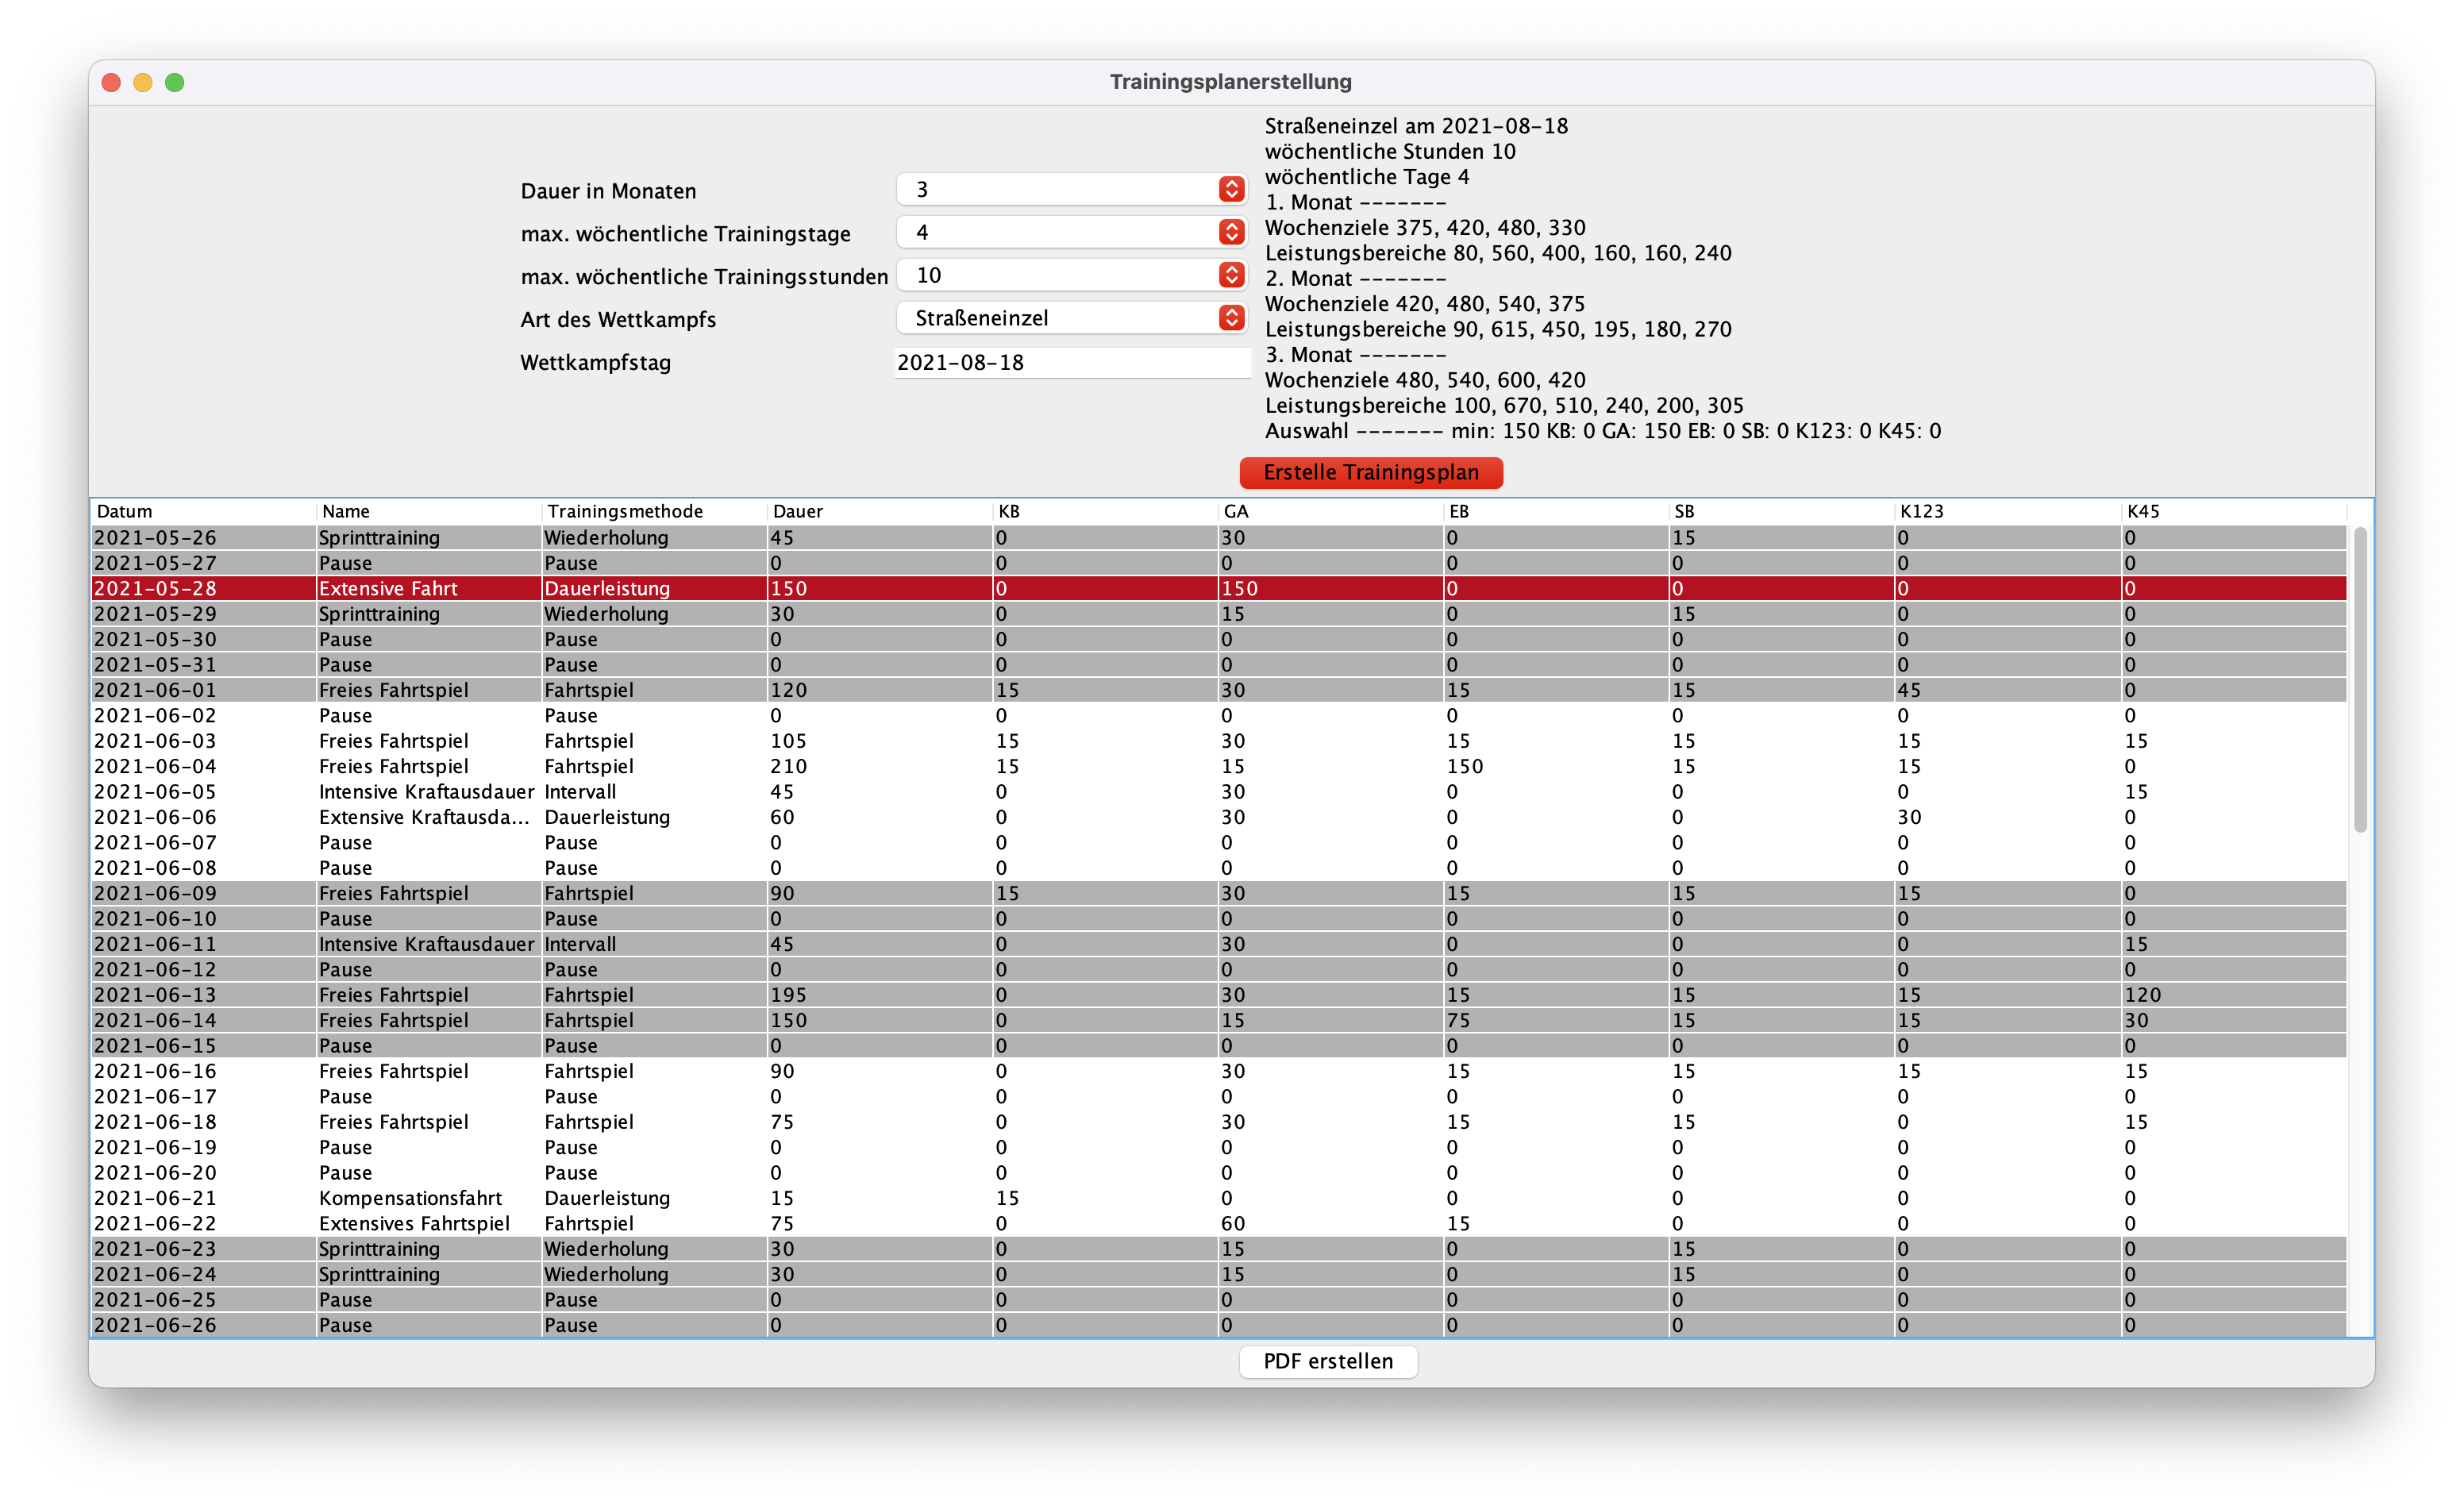
\includegraphics[width=\textwidth]{gfx/gui.png}
    \captionof{figure}{Bildschirmaufnahme der grafischen Oberfläche}
    \end{minipage}
}
\label{anhang:gui}

\newpage
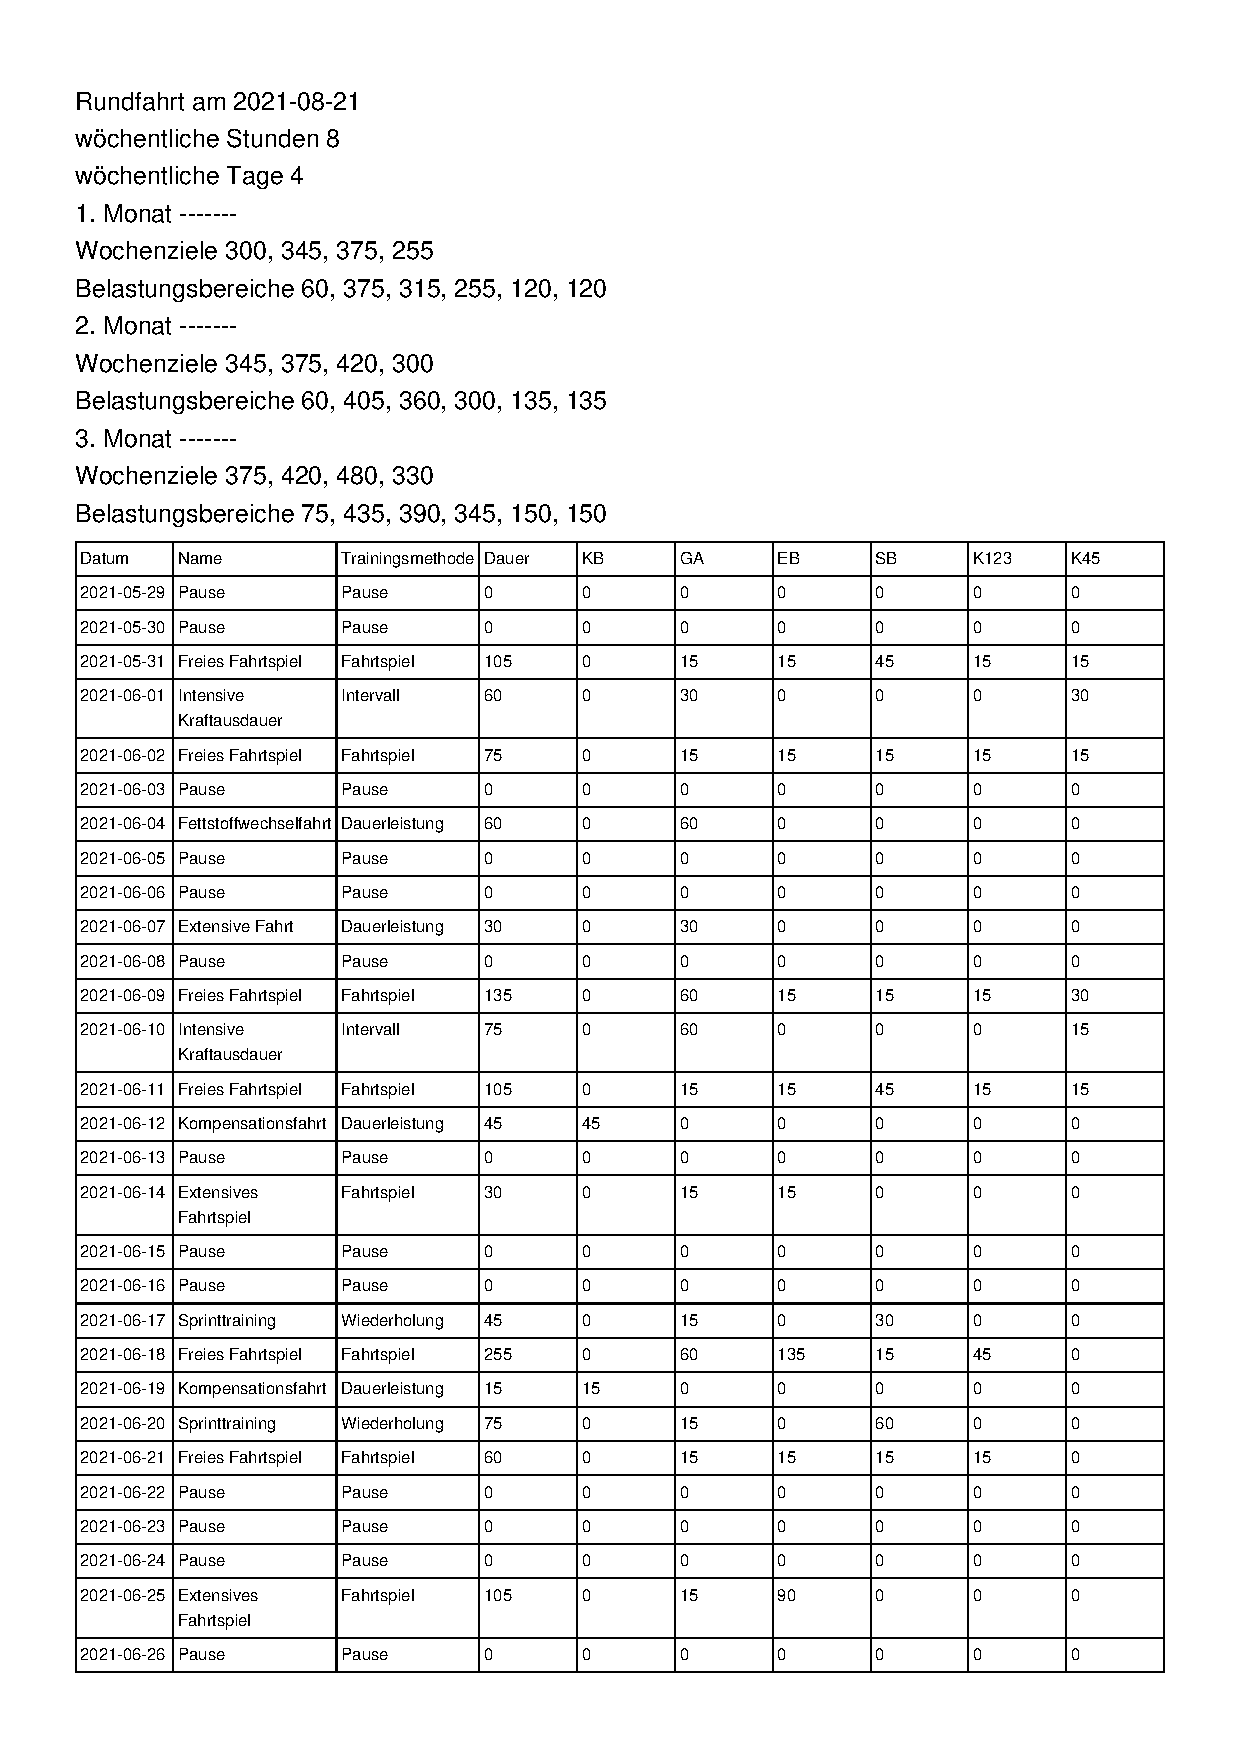
\includepdf[pages=1, scale=0.8, pagecommand=\section{Beispiel Trainingsplan}]{gfx/TimetrialCompetition_4d_8h.pdf}
\label{anhang:beispielplan}
\includepdf[pages=2-, scale=0.8]{gfx/TimetrialCompetition_4d_8h.pdf}

\newpage